%%%%%%%%%%%%%%%%%%%%%%%%%%%%%%%%%%%%%%%%%%%%%%%%%%%%%%%%%%%%%%%%%%%%%%%%%%%%%%%%
% AMS Beamer series / Bologna FC / Template
% Andrea Omicini
% Alma Mater Studiorum - Università di Bologna
% mailto:andrea.omicini@unibo.it
%%%%%%%%%%%%%%%%%%%%%%%%%%%%%%%%%%%%%%%%%%%%%%%%%%%%%%%%%%%%%%%%%%%%%%%%%%%%%%%%
%\documentclass[handout]{beamer}\mode<handout>{\usetheme{default}}
%
\documentclass[presentation, 9pt]{beamer}\mode<presentation>{\usetheme{AMSBolognaFC}}
%\documentclass[handout]{beamer}\mode<handout>{\usetheme{AMSBolognaFC}}
%%%%%%%%%%%%%%%%%%%%%%%%%%%%%%%%%%%%%%%%%%%%%%%%%%%%%%%%%%%%%%%%%%%%%%%%%%%%%%%%
\usepackage[T1]{fontenc}
\usepackage{wasysym}
\usepackage{amsmath,blkarray}
\usepackage[minted,most]{tcolorbox}
\usepackage{centernot}
\usepackage{fontawesome}
\usepackage{fancyvrb}
\usepackage{minted}
\setminted[scala]{baselinestretch=1,obeytabs=true, tabsize=2}
\usepackage[ddmmyyyy]{datetime}
\definecolor{darkcyan}{rgb}{0.0, 0.55, 0.55}
\renewcommand{\dateseparator}{}
%\renewcommand{\thefootnote}{\fnsymbol{footnote}}
\newcommand{\version}{1}
\usepackage[
	backend=biber,
	citestyle=authoryear-icomp,
	maxcitenames=1,
	bibstyle=numeric]{biblatex}

	\makeatletter

\addbibresource{biblio.bib}
%%%%%%%%%%%%%%%%%%%%%%%%%%%%%%%%%%%%%%%%%%%%%%%%%%%%%%%%%%%%%%%%%%%%%%%%%%%%%%%%
\title[Period Abroad Recap]
{Period Abroad Recap}
%
\subtitle[Graph Neural Networks and Spatio-Temporal tracking]
{Graph Neural Networks and Spatio-Temporal tracking}
%
\author[\sspeaker{Aguzzi}]
{\speaker{Gianluca Aguzzi} \href{mailto:gianluca.aguzzi@unibo.it}{gianluca.aguzzi@unibo.it}}
%
\institute[DISI, Univ.\ Bologna]
{Dipartimento di Informatica -- Scienza e Ingegneria (DISI)\\
\textsc{Alma Mater Studiorum} -- Universit{\`a} di Bologna \\[0.5cm]
}
%
\renewcommand{\dateseparator}{/}
\date[\today]{\today}
%
\AtBeginSection[]
{
  \begin{frame}
  \frametitle{Contents}
  \tableofcontents[currentsubsection, 
	sectionstyle=show/shaded, 
	subsectionstyle=show/shaded]
  \end{frame}
}
\AtBeginSubsection[]
{
  \begin{frame}
  \frametitle{Contents}
  \tableofcontents[currentsubsection, 
	sectionstyle=show/shaded, 
	subsectionstyle=show/shaded]
  \end{frame}
}
%%%%%%%%%%%%%%%%%%%%%%%%%%%%%%%%%%%%%%%%%%%%%%%%%%%%%%%%%%%%%%%%%%%%%%%%%%%%%%%%
\begin{document}
%%%%%%%%%%%%%%%%%%%%%%%%%%%%%%%%%%%%%%%%%%%%%%%%%%%%%%%%%%%%%%%%%%%%%%%%%%%%%%%%

%/////////
\frame{\titlepage}
%/////////
%===============================================================================
\section{Introduction}
\begin{frame}{Activities -- One slide}
\begin{itemize}
	\item \bold{Main idea}: spatio-temporal tracking of a natural phenomenon
	\begin{itemize}
		\item Generation of synthetic data (moving boids)
		\item Studying of spatio-temporal neural network models (forecast)
		\begin{itemize}
			\item Graph Neural Networks
			\item Reccurrent Neural Networks
			\item \emph{Recurrent Graph Neural Networks}
		\end{itemize}
		\item Training GNNs through PyTorch and data generated from Alchemist
		\item Integrate Neural networks with Aggregate Computing
		\item Use forecast to compute the best path for nodes
	\end{itemize}
	\item \bold{Clustering}: continue the idea of swarm-based clustering -- avoid the leader election phase
	\begin{itemize}
		\item Inside the cluster, compute the leader (bounded leader election)
	\end{itemize}
\end{itemize}
\end{frame}
%===============================================================================

%===============================================================================
\section{Graph Neural Networks}
\begin{frame}{Artificial Neural Networks -- Recap}
\begin{alertblock}{Definition}
	Collection of units (also called \emph{artificial neuron}) that simulates the behavior of biological neurons
	connected by weighted edges (also called \emph{synapses}).
\end{alertblock}
\begin{itemize}
	\item Typical organization: \emph{input layer}, \emph{hidden layers}, \emph{output layer}
	\item Each layer is composed by a set of neurons
	\item The output of each layer is computed as: $y = f(\sum_{i=1}^n w_i x_i)$ where $f$ is the activation function
	\item The way in which the neurons are connected is called \emph{topology}
	\item The are several topology types:
	\begin{itemize}
		\item Fully connected (MLP): standard neural network, used for classification and regression problem 
		\item Convolutional: used for image processing
		\item Recurrent: used for time series prediction
		\item \bold{Graph Neural Networks}: used for graph processing
	\end{itemize}
\end{itemize}
\end{frame}
%===============================================================================
\begin{frame}{Graph Neural Networks}
\begin{alertblock}{Definition}
	A graph neural network (GNN)~\scite{scarselli2008graph} is a neural network that operates on \textit{graphs}
\end{alertblock}
\begin{itemize}
	\item \bold{Tasks}
	\begin{itemize}
		\item Node classification: given a graph $G=(V,E)$ and a set of labels $X$, predict the label of each node $v \in V$
		\item Link regression: given a graph $G=(V,E)$ and a set of labels $X$, predict the label of each edge $(u,v) \in E$
		\item Graph classification/regression: given a graph $G=(V,E)$ and a set of labels $X$, predict the label of the graph
	\end{itemize}
	\item \bold{Applications}
	\begin{itemize}
		\item \emph{Representation learning}
		\item \emph{Traffic forecast}~\scite{jiang2022graph}
		\item Physics simulations~\scite{jiang2022graph}
		\item Recommandation systems~\scite{wu2020graph}
		\item Chemistry (Molecular fingerprint, chemical reaction)~\scite{zhou2020graph}
		\item Stock market~\scite{matsunaga2019exploring}
		\item Program verification~\scite{NEURIPS2019_49265d24}
		\item ...
	\end{itemize}
	\item Amazing gentle introduction: 
	\begin{itemize}
		\item \url{https://distill.pub/2021/gnn-intro/}
		\item \url{https://tkipf.github.io/graph-convolutional-networks/}
	\end{itemize}
\end{itemize}
\end{frame}

\begin{frame}{GNN structure \& dynamics}
	\begin{itemize}
		\item \bold{Idea}: iteratively update the node representations 
		by combining the representations of their neighbors and their own representations
		\item \bold{K}: layer of GNNs
		\item \bold{$H^i$}: node representations at layer i ($H^0 = X$)
		\item each layer:
		\begin{itemize}
			\item aggregate the information from the neighbors of each node (\textbf{AGGREGATE} phase) $\sim$ \bold{\lstinline|nbr|}
			\item update the node representations by combining the aggregated information from neighbors with the current node representations (\textbf{COMBINE}) $\sim$ \bold{\lstinline|foldhood|}
		\end{itemize}
		\item Matematically:
			$$
			\begin{array}{l}
			a_v^k=\text{AGGREGATE}^k\left\{H_u^{k-1}: u \in N(v)\right\} \\
			H_v^k=\mathbf{COMBINE}^k\left\{H_v^{k-1}, a_v^k\right\},
			\end{array}
			$$
		\item $N(v)$: neighborhood of node $v$
		\item \textbf{AGGREGATE} could be: \textbf{sum}, \textbf{mean}, \textbf{max}, \textbf{min}, \textbf{attention}, etc.
		\item \textbf{COMBINE} could be: \textbf{concatenation}, \textbf{addition}, \textbf{neural network}, etc.
		\item Several architecture are proposed, changing the \textbf{AGGREGATE} and \textbf{COMBINE} functions:
		\begin{itemize}
			\item Graph Convolutional Networks (GCN)~\scite{kipf2016semi}
			\item Graph SAGE~\scite{hamilton2017inductive}
		\end{itemize}
	\end{itemize}
\end{frame}

\begin{frame}[fragile]{GNN structure \& dynamics}
	\centering
	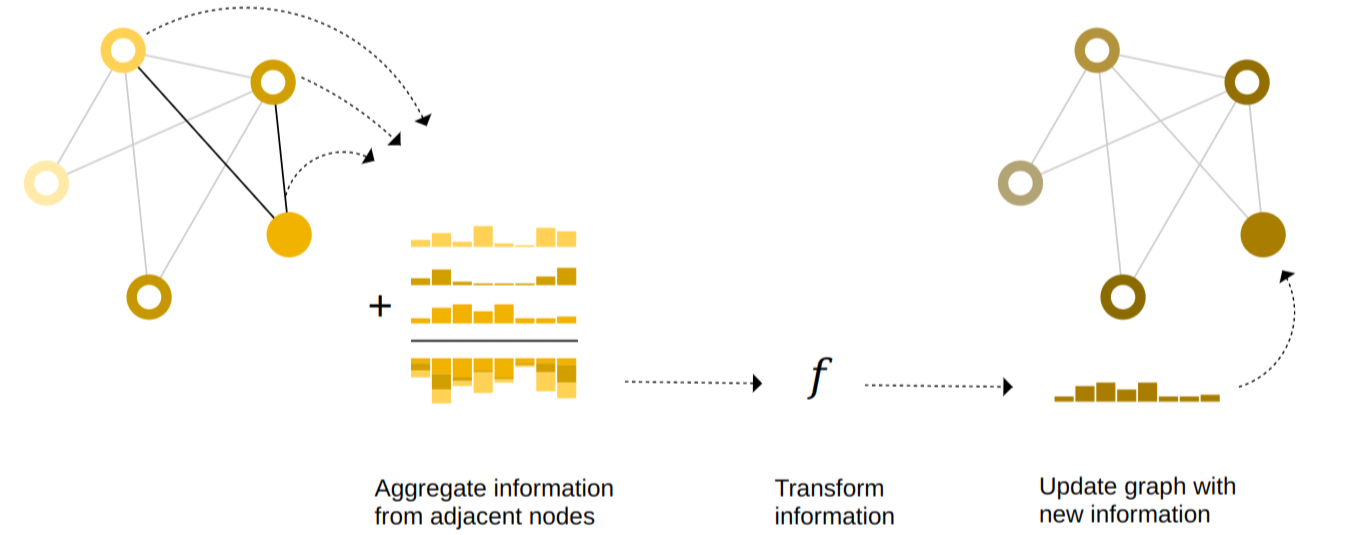
\includegraphics[width=\textwidth]{img/example-gnn.png}

\end{frame}
\begin{frame}{GNN: Aggregate Computing perspective}
	\begin{itemize}
			\item GNN updates the node representations in a \textbf{parallely} {\textcolor{darkcyan}\faThumbsUp} but globally synchronized {\textcolor{bolognafcred}\faThumbsDown}
			\begin{itemize}
				\item Despite that, GNN could be use for distributed computing {\textcolor{darkcyan}\faThumbsUp}
			\end{itemize} 
			\item Stacking several layers of GNNs, lead to several hops of information propagation
			\begin{itemize}
				\item Therefore, we could use at most one layer \faArrowRight \, no deep structure for graph representation
			\end{itemize}
			\item If we consider node-wise computation, GNNs processing does not depend on neighborhood size {\textcolor{darkcyan}\faThumbsUp}
			\item \emph{Learning process}: Centralised Training and Decentralised Execution (CTDE) approach:
			\begin{itemize}
				\item Gather several `snapshots' of the aggregate systems as a graphs
				\begin{itemize}
					\item Features of the nodes: the state of the nodes (sensors, etc.)
					\item Weight of the edges: distances, metric, neighborhood data, etc.
				\end{itemize}
				\item Train a GNN on the gathered graphs
				\item `Deploy' the GNN on the aggregate systems
				\begin{itemize}
					\item Each node executes the GNN locally sharing the same parameters (homegenous behaviour)
				\end{itemize}
			\end{itemize}
			\item Potential limitations:
			\begin{itemize}
				\item Synchronized update \faArrowRight \, each node should wait the update of its neighbors
				\item Dynamic graph: GNN learn structural relation, no temporal relation (e.g., neighborhood changes, etc.)
			\end{itemize}
		\end{itemize}
\end{frame}
\begin{frame}[fragile]{Towards Timeseries forecast using GNN}
\begin{itemize}
	\item GNN are typically used for static graphs
	\begin{itemize}
		\item connection doesn't change over time
		\item single snapshot of the graph is enough to predict the label
	\end{itemize}
	\item Recent works try to use GNN for timeseries prediction \faArrowRight \, spatio temporal neural networks
	\begin{itemize}
		\item Distributed controller for robots ~\scite{tolstaya2020learning}
		\item Trafic forecast~\scite{zhao2019t}
		\item Weather forecast~\scite{keisler2022forecasting}
	\end{itemize}
	\item Simple Idea: stack GNN structure with a recurrent neural network (RNN) -- or network with memory capabilities
	\item Conceptually, the RNN could be applied in each node performing a local update on its own state
	\begin{itemize}
		\item The state depends on the neighborhood since it is the outpud of the GNN
	\end{itemize}	
	\centering
\end{itemize}
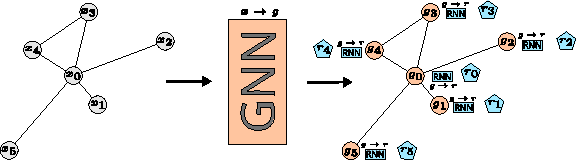
\includegraphics[width=\textwidth]{img/idea.pdf}

\end{frame}
%===============================================================================
\section{Aggregate Computing + Neural Networks}
%===============================================================================
\begin{frame}[fragile, allowframebreaks]{Aggregate Computing \faPlus \, Neural Networks: Integration perspective}
\begin{itemize} 
	\item Neural networks can be seen as simple functions
	\begin{itemize}
		\item Some of them should be carefully considered (how to deal with time series? how to deal with graphs?)
	\end{itemize}
	\item In the following, we consider a general schema in how to applied NNs in AC
	\item I don't cover the learning process -- I consider that it is already done using an external process
	\begin{itemize}
		\item \mintinline{scala}|sense("feature")| get the feature of interest
		\item \mintinline{scala}|nbrData| get the associated with the weighted neighborhood
		\item \mintinline{scala}|NN| is the function associated with the neural network
	\end{itemize}
\end{itemize}
\begin{alertblock}{MLP}
No need to handle time or spatial aspects
\begin{minted}{scala}
def main() = NN(sense("feature"))
\end{minted}
\end{alertblock}
\begin{alertblock}{RNN}
Similarly as MLP, but you need to use \mintinline{scala}|rep| to encode the temporal aspect
\begin{minted}{scala}
def main() = 
	rep(default){
		memory => NN(sense("feature"), memory)
	}
\end{minted}
\end{alertblock}
\begin{alertblock}{GNN}
	In this case case you need to use \mintinline{scala}|nbr| in order to build the local graph-view
\begin{minted}{scala}
def main() = 
	val neighborhoodFeature = includingSelf(nbr(sense("feature")))
	val neighborhoodWeight = excludingSelf(nbrData)
	NN(neighborhoodFeature, neighborhoodWeight)
\end{minted}
NB! The order of the feature vector and the weigtht should be preserved
\end{alertblock}
\begin{alertblock}{GNN \faPlus \, RNN}
	You need to use \mintinline{scala}|rep| and \mintinline{scala}|nbr| in order to build the local graph-view with memory
\begin{minted}{scala}
def main() =
	rep(default){
		memory => 
			val neighborhoodFeature = includingSelf(nbr(sense("feature")))
			val neighborhoodWeight = excludingSelf(nbrData)
			val nbrMemory = includingSelf(nbr(memory))
			NN(neighborhoodFeature, neighborhoodWeight, nbrMemory)
	}
\end{minted}
NB! Some NNs use as input the neighborhood memory information
\end{alertblock}
\end{frame}

%===============================================================================
\section{Use case: spatio temporal forecast + tracking}
%===============================================================================


%===============================================================================
\section{Clustering}
%===============================================================================


%===============================================================================
\section*{}
%===============================================================================

%/////////
\frame{\titlepage}
%/////////

%===============================================================================
\section*{\refname}
%===============================================================================

%%%%
\setbeamertemplate{page number in head/foot}{}
%/////////
\begin{frame}[c,noframenumbering, allowframebreaks]{\refname}
%\begin{frame}[t,allowframebreaks,noframenumbering]{\refname}
	\tiny
	\printbibliography
\end{frame}
%/////////

%%%%%%%%%%%%%%%%%%%%%%%%%%%%%%%%%%%%%%%%%%%%%%%%%%%%%%%%%%%%%%%%%%%%%%%%%%%%%%%%
\end{document}
%%%%%%%%%%%%%%%%%%%%%%%%%%%%%%%%%%%%%%%%%%%%%%%%%%%%%%%%%%%%%%%%%%%%%%%%%%%%%%%%
